\documentclass[11pt]{article}

\usepackage{microtype}
\usepackage{rotating,booktabs}
\usepackage{geometry} %\usepackage[showframe]{geometry}
\usepackage{tabularx}
\usepackage[backend=bibtex]{biblatex}
\usepackage{graphicx}
\usepackage{caption,subcaption}
\usepackage{float}
\usepackage[hidelinks]{hyperref}


\DeclareGraphicsExtensions{.pdf,.png,.jpg}


\usepackage{Sweave}
\begin{document}
\input{TaaS-concordance}

\title{\href{http://vvkmnn.wordpress.com/2014/06/12/saas-and-r/}{Ties as a Service}}
\author{\href{http://vvkmnn.wordpress.com/}{Vivek Menon}}
\date{June 2014}
\maketitle

\bigskip\bigskip\bigskip
\bigskip\bigskip\bigskip
\bigskip\bigskip\bigskip


\begin{abstract}
A predictive analysis of the 'Monthly Recurring Revenue' (MRR) model, which allows for the customer to be treated a series of recurring transactions instead of a single transaction, and is thus often employed when describing  the behavior of 'Software as a Service' (SaaS) firms. This  analysis is based on thousands of randomly generated independent and identically distributed simulations using a variation of the Monte Carlo method.

\begin{center}
\textbf{Scenario}: Best 
\end{center}
\end{abstract}




\newpage


\section*{Introduction}

\subsection*{Premise}
This work sets out to create a coherent, reproducible Monte Carlo simulation of the MRR Model in the context of SaaS firms. It uses the fictional 'Ties as a Service' business to contextualize the data and illustrate the framework. All assumptions and interpretations herein are conjectured.  Relevant references are hyperlinked.

\subsection*{Background}

\subsubsection*{MRR}

In this report, we will attempt to understand and simulate the features of the MRR model, as described by David Skok\footnote{\href{http://www.forentrepreneurs.com/saas-metrics-2/}{'SaaS Metrics 2.0 - A Guide to Measuring and Improving what Matters'}} in his analysis of SaaS businesses. The principle basis of this model is the idea of 'recurring revenue'; that a customer will continue paying for an offered service over time. This is not dissimilar to the idea of a recurring subscription, monthly fees, or annual contracts. 


\subsubsection*{SaaS}

SaaS is considered part of the nomenclature of the Cloud Computing industry. "Examples of SaaS include enterprise-level applications such as Salesforce, Netsuite ... Google Apps to personal applications such as
GMail, TurboTax Online, Facebook, or Twitter".\footnote{\href{http://www.sciencedirect.com/science/article/pii/S0167923610002393}{'Cloud computing - The business perspective'}} It is essentially a system whereby a consumer subscribes to a particular software or service, in lieu of purchasing versions of it on a transactiational basis. This contractual format allows the end user to use their software locally on a myriad of devices while the majority of the computing and processing takes place offsite. One noteable example of such a service is Hootsuite, which offers a subscription-based social media management service:
\begin{center}
\href{http://www.hootsuite.com}{
\includegraphics[width=3cm]{HootSuite.png}}
\end{center}


\newpage

\subsection*{Company Overview}

\begin{center}

\includegraphics[width=3cm]{Tie.png}
\end{center}

\begin{center}
\textbf{Ties as a Service}
\end{center}


"Ties as a Service" is a fictional business that will be used to simulate the behavior of the 'Software as a Service' business model. It is similiar to the "Jerky as a Service" model by Noah Kagan\footnote{\href{http://www.appsumo.com/sumo-jerky/}{'The results of the 24-Hour Business Challenge'}}, which was used as a basis to generate comparable numbers. 

The business operates under the following assumptions:

\begin{enumerate}
  \item For a monthly subscription of \$$30$, the client recieves 2 random ties every month. 
  \item The Average Revenue per Account (ARPA) is therefore \$$30$ inititally.
  \item The profit margin on every sale is $45$\%.
  \item The initial customer base is assumed to be $60$.
  \item The initial Monthly Recurring Revenue (MRR) therefore is \$$1800$.
  \item The discount rate\footnote{\href{http://www.investopedia.com/terms/d/discountrate.asp}{'Discount Rate - Investopedia'}} is assumed to be $10$\%.
  \item The initial advertising budget for this firm is assumed to be \$$300$ monthly.
\end{enumerate}

\newpage

\section*{Methodology}

The MRR model is affected by two key factors; Customer Churn \& Growth and Revenue Churn \& Growth. 'Churn' is the notion of loss over time; it is the factor by which a firm's customer base or MRR is eroded by customers leaving the firm or downgrading their subscription. Growth refers to the rate at which the firm acquires new customers or clients upgrade their service. 

For the purposes of this example, this business has only 1 tier of service. In practice, this assumption is important, as losing 10 customers can be very different depending on what tiers you lose them from. For example, one could lose $9 \cdot \$100$ accounts and $1 \cdot \$1000$ account, or lose $5 \cdot \$100$ accounts and $5 \cdot \$1000$ accounts, which have different effects on the MRR of a firm. However,it is assumed in this example that all customers are equally valuable. 

Let us also assume that the Churn and Growth rates are randomly generated values that are distributed according to the following means and variations.  


% latex table generated in R 3.1.1 by xtable 1.7-3 package
% Mon Jul 28 20:14:43 2014
\begin{table}[ht]
\centering
\begin{tabular}{rll}
  \hline
 & Mean & SD \\ 
  \hline
Churn & 2 \% & 2 \% \\ 
  Growth & 7 \% & 2 \% \\ 
   \hline
\end{tabular}
\caption{Summary of Customer Variation} 
\end{table}
Using these values, it is possible for us to create randomly generated Churn \& Growth vectors, so that we can then analyze how the following functions change over time.

\newpage

\subsection*{Functions}




\subsubsection*{Customers}

The Customers ($C_{1}, C_{2}, \ldots, C_{n}$) are the basis for the MRR model, and is usually the key measure of any SaaS business. It changes as a result of New Customers acquired over time ($NC_1, NC_2, \ldots, NC_n$) and Churned Customers over time ($CC_{1}, CC_{2}, \ldots, CC_{n}$). Therefore, it can be related to the Customer Churn factor, ($c_{i}$) and the Customer Growth factor, ($g_{i}$) in the following way:

\[
C_{i+1} = C_{i} + NC_{i+1} - CC_{i+1}
\]
\[
C_{i+1} = C_{i}(1 + g_{i} - c_{i})
\]


\subsubsection*{Subscription}

The Subscription ($S_{1}, S_{2}, \ldots, S_{n}$) is the next key value of the MRR model. It represents the Monthly Subscription rate, here \$$30$. This value is usually determined by the firm, and is therefore typically independent of the other functions. 

\[
S_{i}
\]

\subsubsection*{MRR}

The MRR ($MRR_{1}, MRR_{2}, \ldots, MRR_{n}$) is the Monthly Recurring Revenue. It changes as a function of customers and the monthly subscription rate ($S_{i}$):

\[
MRR_{i} = C_{i} \cdot S_{i}
\]

\subsubsection*{ARPA}

The ARPA ($ARPA_{1}, ARPA_{2}, \ldots, ARPA_{n}$) is a function of the MRR and Customers, and measures what the Average Revenue per Accout for a given period. It changes as a function of Customers ($C_{i}$) and the monthly subscription rate ($S_{i}$):

\[
ARPA_{i+1} = \frac{(C_{i} \cdot ARPA_{i}) + ((NC_{i+1} - CC_{i+1}) \cdot S_{i+1})}{C_{i+1}}
\]


\subsubsection*{LTV}

The LTV ($LTV_{1}, LTV_{2}, \ldots, LTV_{n}$) is the Lifetime Value of a Customer, and determines how much the 'lifetime' cash flow of a Customer acquired in any period $i$  is. Here, the Customer lifetime can be calculated by realizing that the Churn factor $c_{i}$ represents the monthly rate at which a specific monthly cohort exhausts itself. Therefore, $\frac{1}{c_{i}}$ is the amount of months it takes for a Cohort to exhaust itself, and similarly, the number of periods we need to discount this cashflow by the discount rate 10\%. 

For the sake of accuracy, we also apply the Profit Margin ($PM_{i}$), here 45\% to the ARPA in order to account for profit exclusively:

\[
LTV_{i} = \frac{ARPA_{i} \cdot PM_{i} \cdot \frac{1}{c_{i}}}{(1 + \frac{r}{\frac{1}{c_{i}}}))^\frac{1}{c_{i}}}
\]


\subsubsection*{CAC}

The CAC ($CAC_{1}, CAC_{2}, \ldots, CAC_{n}$) is the Cost to Acquire a Customer, and determines how much the cost to acquire each New Customer was for any period $i$  . It is a function of the Advertising Budget ($AB_{i}$), here \$300, and the number of New Customers ($NC_{i}$). 


\[
CAC_{i} = \frac{AB_{i}}{NC_{i}}
\]


\subsubsection*{CAC Recovery}

The CAC Recovery ($CACr_{1}, CACr_{2}, \ldots, CACr_{n}$) is the measure of the Months it would take to recover the Cost to Acquire a Customer in any period $i$  given the firm's profit. It is a function of the Cost to Acquire a Customer ($CAC_{i}$), the monthly subscription rate ($S_{i}$), here \$30, and the Profit Margin ($PM_{i}$), here 45\%:


\[
CACr_{i} = \frac{CAC_{i}}{S_{i} \cdot PM_{i}}
\]

\subsubsection*{LTV/CAC}

The LTV/CAC ($\frac{LTV}{CAC}_{1}, \frac{LTV}{CAC}_{2}, \ldots, \frac{LTV}{CAC}_{n}$) is the ratio of the Lifetime Value to the Cost to Acquire a Customer, and determines how much a customer is worth over his entire lifetime in terms of the cost taken to acquire him in any period $i$  is. It is a function of the LTV ($LTV_{i}$), and the CAC ($CAC_{i}$):


\[
\frac{LTV}{CAC}_{i} = \frac{LTV_{i}}{CAC_{i}}
\]

\newpage

\section*{Simulation}

\subsection*{Generation}

Therefore, using these functions, and a randomly generated expected Customer Churn and expected Customer Growth, it is possible to simulate a variety of "random walk" cases that allow us to simulate a variety of future scenarios using the Monte Carlo method. Table \ref{tabcp} and  Table \ref{tabmp} are the mean vectors that result from running these functions on 5001 \textit{i.i.d.} random samples. 


% latex table generated in R 3.1.1 by xtable 1.7-3 package
% Mon Jul 28 20:25:43 2014
\begin{table}[ht]
\centering
\begin{tabularx}{\textwidth}{rrrrr}
  \hline
 & Customers & Churned Customers & New Customers &  Customer Change \\ 
  \hline
January & 60.00 & 1.40 & 4.21 & 2.82 \\ 
  February & 62.82 & 1.45 & 4.35 & 2.90 \\ 
  March & 65.72 & 1.55 & 4.60 & 3.05 \\ 
  April & 68.77 & 1.61 & 4.81 & 3.20 \\ 
  May & 71.97 & 1.70 & 5.04 & 3.34 \\ 
  June & 75.31 & 1.74 & 5.28 & 3.55 \\ 
  July & 78.86 & 1.83 & 5.51 & 3.67 \\ 
  August & 82.53 & 1.93 & 5.76 & 3.83 \\ 
  September & 86.36 & 2.00 & 6.06 & 4.06 \\ 
  October & 90.42 & 2.10 & 6.31 & 4.21 \\ 
  November & 94.64 & 2.20 & 6.61 & 4.41 \\ 
  December & 99.05 & 2.31 & 6.96 & 4.66 \\ 
   \hline
\end{tabularx}
\caption{Customer Projections} 
\label{tabcp}
\end{table}
% latex table generated in R 3.1.1 by xtable 1.7-3 package
% Mon Jul 28 20:25:43 2014
\begin{table}[ht]
\centering
\begin{tabularx}{\textwidth}{rrrrrrrr}
  \hline
 & Subscription & MRR & ARPA & LTV & CAC & Recover CAC & LTV/CAC \\ 
  \hline
January & 30.00 & 1800.00 & 30.00 & 3381.70 & 79.03 & 5.85 & 52.21 \\ 
  February & 30.00 & 1884.46 & 30.00 & 2671.67 & 79.03 & 5.85 & 37.78 \\ 
  March & 30.00 & 1971.54 & 30.00 & 2830.55 & 79.03 & 5.85 & 39.63 \\ 
  April & 30.00 & 2063.06 & 30.00 & 2764.45 & 79.03 & 5.85 & 35.17 \\ 
  May & 30.00 & 2159.11 & 30.00 & 2377.92 & 79.03 & 5.85 & 32.63 \\ 
  June & 30.00 & 2259.37 & 30.00 & 2866.01 & 79.03 & 5.85 & 38.37 \\ 
  July & 30.00 & 2365.72 & 30.00 & 2669.70 & 79.03 & 5.85 & 36.32 \\ 
  August & 30.00 & 2475.86 & 30.00 & 3795.27 & 79.03 & 5.85 & 50.47 \\ 
  September & 30.00 & 2590.82 & 30.00 & 9153.33 & 79.03 & 5.85 & 122.21 \\ 
  October & 30.00 & 2712.69 & 30.00 & 3490.63 & 79.03 & 5.85 & 49.10 \\ 
  November & 30.00 & 2839.08 & 30.00 & 2831.38 & 79.03 & 5.85 & 39.69 \\ 
  December & 30.00 & 2971.51 & 30.00 & 3760.61 & 79.03 & 5.85 & 45.12 \\ 
   \hline
\end{tabularx}
\caption{MRR Projections} 
\label{tabmp}
\end{table}




\newpage
\subsection*{Visualization}



However, the MRR model is most intuitively analyzed in terms of Cohorts, where t is much easier to see the erosion and expansion of each individual group of New Customers. Table \ref{tabcc} and  Table \ref{tabmc} are the Cohort tables that result from running this simulation 5001 times. 


% latex table generated in R 3.1.1 by xtable 1.7-3 package
% Mon Jul 28 20:25:43 2014
\begin{table}[ht]
\centering
\scalebox{0.75}{
\begin{tabular}{rrrrrrrrrrrrr}
  \hline
 & January & February & March & April & May & June & July & August & September & October & November & December \\ 
  \hline
1 & 60 & 58 & 56 & 55 & 54 & 52 & 52 & 51 & 51 & 50 & 49 & 49 \\ 
  2 & 0 & 5 & 5 & 5 & 5 & 5 & 5 & 5 & 5 & 5 & 5 & 5 \\ 
  3 & 0 & 0 & 2 & 2 & 2 & 2 & 2 & 2 & 2 & 2 & 2 & 2 \\ 
  4 & 0 & 0 & 0 & 4 & 4 & 4 & 4 & 4 & 4 & 4 & 4 & 4 \\ 
  5 & 0 & 0 & 0 & 0 & 5 & 5 & 5 & 4 & 4 & 4 & 4 & 4 \\ 
  6 & 0 & 0 & 0 & 0 & 0 & 5 & 5 & 5 & 5 & 5 & 5 & 4 \\ 
  7 & 0 & 0 & 0 & 0 & 0 & 0 & 7 & 7 & 7 & 7 & 7 & 7 \\ 
  8 & 0 & 0 & 0 & 0 & 0 & 0 & 0 & 6 & 6 & 6 & 6 & 6 \\ 
  9 & 0 & 0 & 0 & 0 & 0 & 0 & 0 & 0 & 5 & 5 & 5 & 5 \\ 
  10 & 0 & 0 & 0 & 0 & 0 & 0 & 0 & 0 & 0 & 6 & 6 & 6 \\ 
  11 & 0 & 0 & 0 & 0 & 0 & 0 & 0 & 0 & 0 & 0 & 9 & 9 \\ 
  12 & 0 & 0 & 0 & 0 & 0 & 0 & 0 & 0 & 0 & 0 & 0 & 9 \\ 
   \hline
\end{tabular}
}
\caption{Customer Cohort Projections} 
\label{tabcc}
\end{table}% latex table generated in R 3.1.1 by xtable 1.7-3 package
% Mon Jul 28 20:25:43 2014
\begin{table}[ht]
\centering
\scalebox{0.7}{
\begin{tabular}{rrrrrrrrrrrrr}
  \hline
 & January & February & March & April & May & June & July & August & September & October & November & December \\ 
  \hline
1 & 1800.00 & 1726.56 & 1677.77 & 1638.65 & 1619.18 & 1570.35 & 1566.15 & 1544.02 & 1519.05 & 1488.66 & 1480.94 & 1471.10 \\ 
  2 & 0.00 & 158.66 & 154.17 & 150.58 & 148.79 & 144.30 & 143.92 & 141.88 & 139.59 & 136.79 & 136.09 & 135.18 \\ 
  3 & 0.00 & 0.00 & 64.29 & 62.79 & 62.04 & 60.17 & 60.01 & 59.16 & 58.21 & 57.04 & 56.75 & 56.37 \\ 
  4 & 0.00 & 0.00 & 0.00 & 130.52 & 128.97 & 125.08 & 124.75 & 122.98 & 121.00 & 118.57 & 117.96 & 117.18 \\ 
  5 & 0.00 & 0.00 & 0.00 & 0.00 & 140.04 & 135.82 & 135.45 & 133.54 & 131.38 & 128.75 & 128.08 & 127.23 \\ 
  6 & 0.00 & 0.00 & 0.00 & 0.00 & 0.00 & 143.19 & 142.81 & 140.79 & 138.51 & 135.74 & 135.04 & 134.14 \\ 
  7 & 0.00 & 0.00 & 0.00 & 0.00 & 0.00 & 0.00 & 223.98 & 220.82 & 217.25 & 212.90 & 211.79 & 210.39 \\ 
  8 & 0.00 & 0.00 & 0.00 & 0.00 & 0.00 & 0.00 & 0.00 & 178.66 & 175.77 & 172.25 & 171.36 & 170.22 \\ 
  9 & 0.00 & 0.00 & 0.00 & 0.00 & 0.00 & 0.00 & 0.00 & 0.00 & 144.81 & 141.92 & 141.18 & 140.24 \\ 
  10 & 0.00 & 0.00 & 0.00 & 0.00 & 0.00 & 0.00 & 0.00 & 0.00 & 0.00 & 194.86 & 193.85 & 192.56 \\ 
  11 & 0.00 & 0.00 & 0.00 & 0.00 & 0.00 & 0.00 & 0.00 & 0.00 & 0.00 & 0.00 & 276.61 & 274.77 \\ 
  12 & 0.00 & 0.00 & 0.00 & 0.00 & 0.00 & 0.00 & 0.00 & 0.00 & 0.00 & 0.00 & 0.00 & 264.24 \\ 
   \hline
\end{tabular}
}
\caption{MRR Cohort Projections} 
\label{tabmc}
\end{table}
The individual trends in these Cohort Tables become more apparent when examined visually in Figure \ref{fig5} and Figure \ref{fig6}. In Figure \ref{fig1}, we can see how the Churn factor, roughly 2\% monthly, erodes each Customer cohort over time. In Figure \ref{fig2} we can examine the cumulative effect of these Cohorts, which the firm acquires at the growth rate of roughly 7\% monthly. Based on the strength of these factors, a typical SaaS business may grow or contract, and exhibit varying behavior over time. 

In Figure \ref{fig3}, we can see the growth and churn of each MRR Cohort over time. In Figure \ref{fig4} we can examine the Cumulative MRR, and see how the business is performing over time. In this simple case, MRR is simply a function of Customer variation, not Revenue Growth or Churn, and is therefore primarily a reflection of Customer behavior. The average Customer Cohort lasts 1557 months.

\begin{figure}
\centering
\begin{subfigure}{0.70\textwidth}
\centering
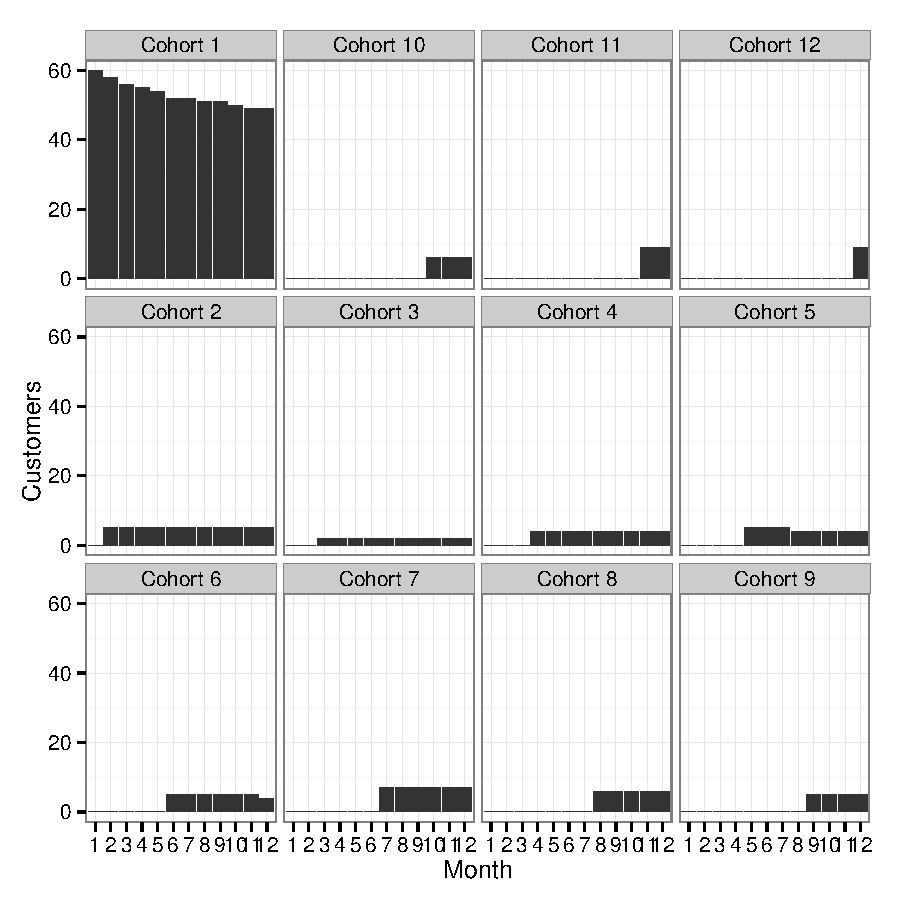
\includegraphics{TaaS-011}
\caption{Customer Cohorts over Time}
\label{fig1}
\end{subfigure}
\begin{subfigure}{0.70\textwidth}
\centering
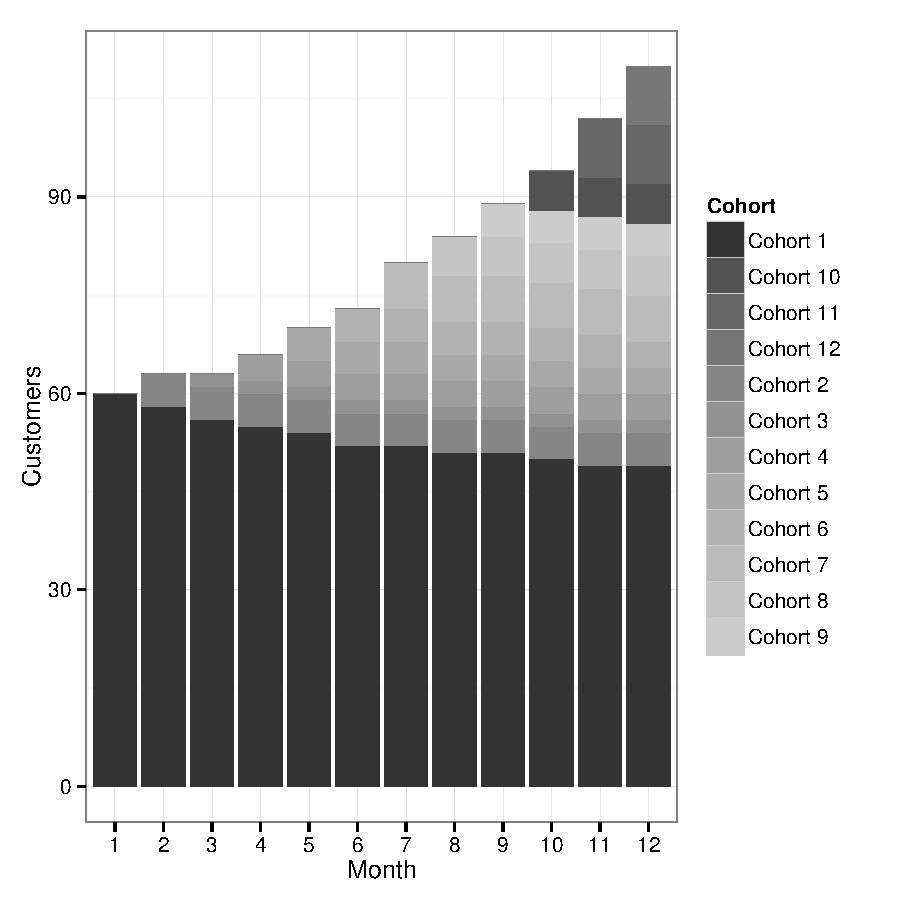
\includegraphics{TaaS-012}
\caption{Cumulative Customers over Time}
\label{fig2}
\end{subfigure}
\caption{Customer Cohorts}
\label{fig5}
\end{figure}


\begin{figure}
\centering
\begin{subfigure}{0.70\textwidth}
\centering
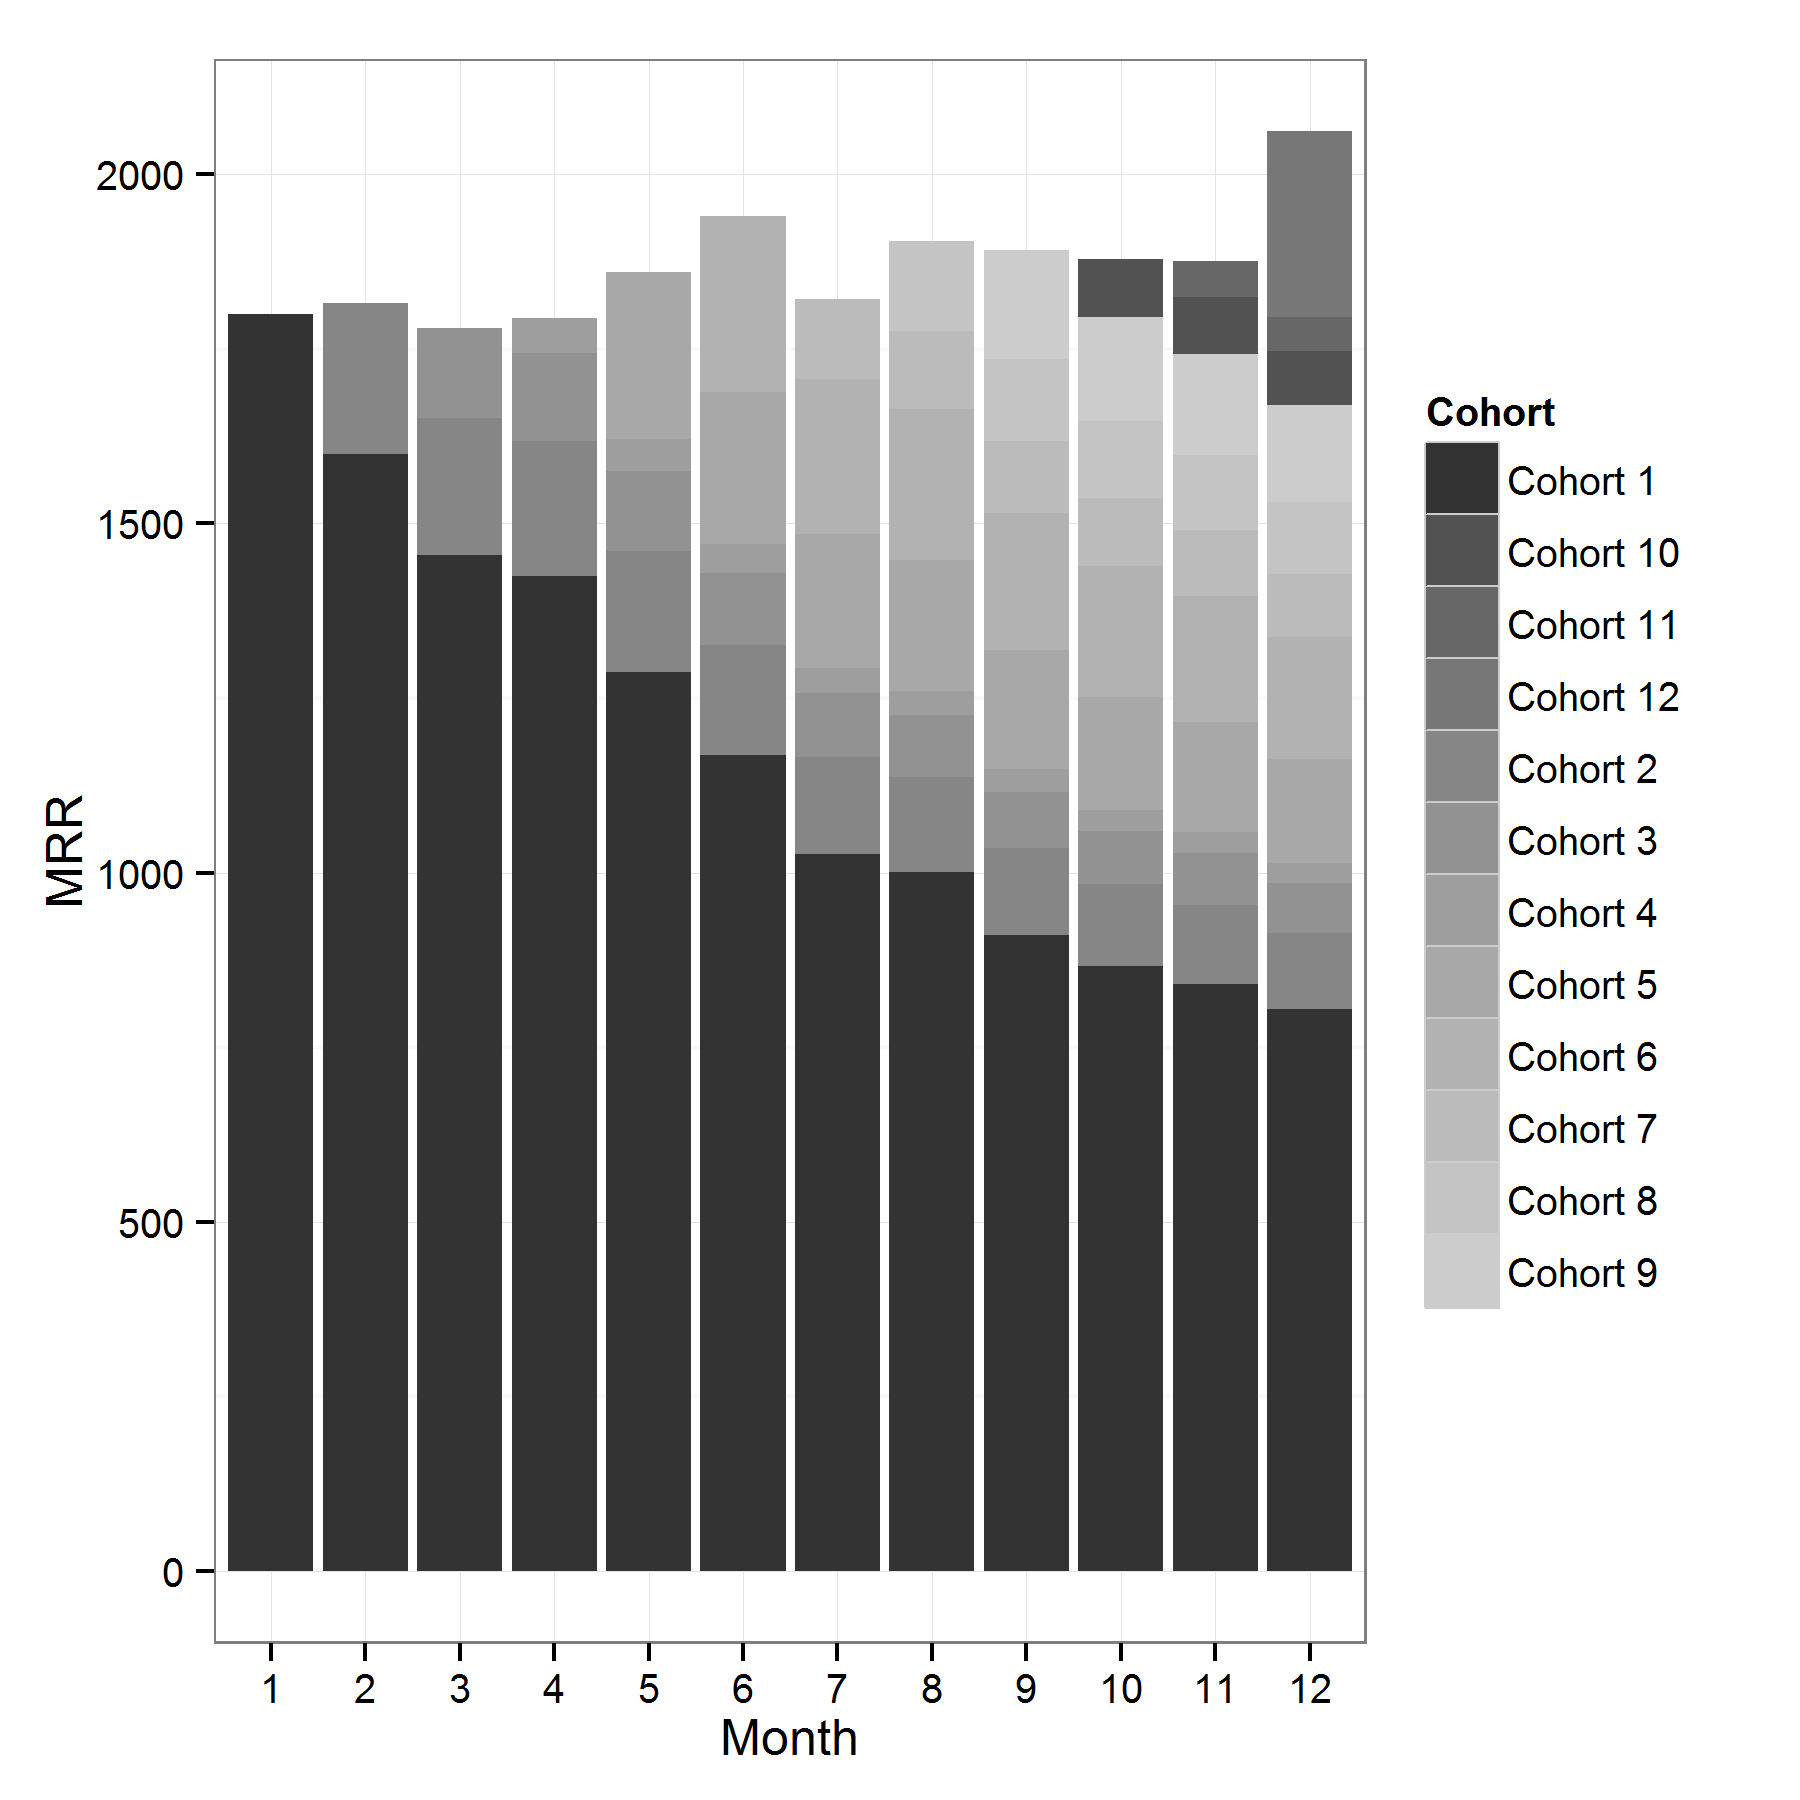
\includegraphics{TaaS-013}
\caption{MRR Cohorts over Time}
\label{fig3}
\end{subfigure}
\begin{subfigure}{0.70\textwidth}
\centering
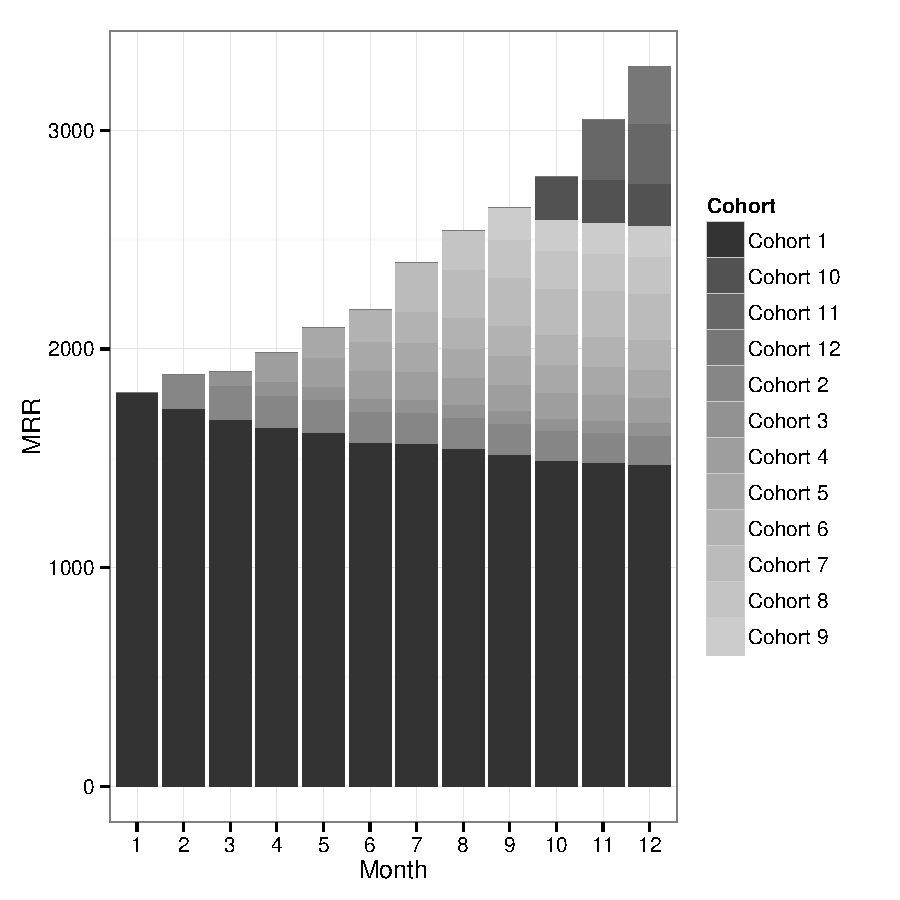
\includegraphics{TaaS-014}
\caption{Cumulative MRR over Time}
\label{fig4}
\end{subfigure}
\caption{MRR Cohorts}
\label{fig6}
\end{figure}

\newpage

\section*{Discussion}

\subsection*{Revenue Churn \& Growth}

It is possible to design a model that takes MRR variation into consideration, but such a model would require different 'tiers' of subscriptions for Customers to move in-between. This would allow Customers to 'upgrade' and 'downgrade', which, coupled with the creation of new contracts for different kinds of New Customers and cancelations of contracts for different kinds of Churned Customers, would cause significant fluctuation in the Monthly Recurring Revenue.  

Thus, we can interpret Revenue Churn and Revenue Growth simply as a Tier weighted function of Churned Customers and New Customers\footnote{\href{http://chaotic-flow.com/what-is-mrr-churn-saas-metrics-faqs-part-2/}{'What is MRR Churn?'}}. In the general case, where $j$ is the number of tiers of subscription:

\[
rc_{i,j} =  \frac{\sum_{n}^{j=1}S_{i,j} \cdot CC_{i,j}}{\sum_{n}^{j=1}S_{i,j} \cdot C_{i,j}} = \frac{\sum_{n}^{j=1}S_{i,j}C_{i,j}(c_{i})}{\sum_{n}^{j=1}S_{i,j}{C_{i,j}}}
\]

\[
rg_{i,j} =  \frac{\sum_{n}^{j=1}S_{i,j} \cdot NC_{i,j}}{\sum_{n}^{j=1}S_{i,j} \cdot C_{i,j}} = \frac{\sum_{n}^{j=1}S_{i,j}C_{i,j}(g_{i})}{\sum_{n}^{j=1}S_{i,j}{C_{i,j}}}
\]

Consider the following attempt to solve for $rc_{5,2}$, or the Revenue Churn on the 5th day for a 2-tier service:

for $i = 5$, $j = {2}$
 \[
 rc_{5,2} = \frac{(S_{5,1} \cdot CC_{5,1}) + (S_{5,2} \cdot CC_{5,2})}{S_{5,2} \cdot C_{5,2} + S_{5,2} \cdot C_{5,2}}
 \]

Thus, given the price of the different Subscription tiers ($S_{i,1}, S_{i,2}, \ldots, S_{i,j}$) and the fluctuation of the Customers in those tiers ($C_{i,1}, C_{i,2}, \ldots, C_{i,j}$), it is possible to examine the fluctuation in MRR over time. 

However, since TaaS has only 1 tier of subscription, such variation has not been analyzed in this version of this paper. As one can see, to do so would require an entire extra dimension of description, which while definitely possible, was impractical given the timeline for this paper.

\subsection*{Parametrization}

This work is capable of generating completely new random vectors, data, tables, figures, and a CSV Dataset of values given different input paramaters in order to examine different scenarios. For an illustration of this feature, please examine the differences in the inputs and results between the 'Best', 'Neutral', and 'Worst' scenarios of this document. 

\newpage

\section*{Conclusion}

These tools and methodologies, have determined a way to use Random Walk theory and Monte Carlo-esque simulations to model this new Marketing theory. The MRR Subscription model has many differences from other traditional models, but it's primary feature is the fact that its customers cannot be treated as a single transaction, but as a series of recurring transactions.

In this way, these Customer cohorts are similar to the idea of Asset cash flows, as used in Financial modeling. Each customer is a 'revenue stream', whose value must be measured over their entire life, instead of just intertemporal snapshots. Furthermore, by discounting this revenue stream to the present, it is possible to understand how much each individual customer is worth to the firm at the present moment, and take steps to improve and profit from that number.

However, while discounting cashflows is relatively trivial, predicting customer behavior is not. One approach is using a means of simulation that accounts for some natural 'noise' via geometric brownian motion and a variety of input paramaters.This model is then capable of simulating thousands of potential scenarious, including an average 'expected' outcome. However, using this methodology to generate results is only a predictive simulation, and may not reflect the actual behavior of real market conditions, which includes significantly more noise and influential factors. 

This method also allows us to simulate a variety of future cases given only a few input variables. During my original upload, I uploaded 3 different versions of this paper, including a 'Best', 'Neutral' , and 'Worst' scenario analysis. All of these analyses were generated from a single file, which included all the code, plots, and PDF formatting, which can be repeated \textit{ad infinitum} for almost any scenario, and improved upon in the future. 

This 'living document' allows for reproduceable research, and an all-inclusive method of report generation and case analysis. This will allow us to generate analysis for 'Ties as a Service' in a a variety of different scenarios, and account for different input paramaters. 

\subsection*{Future}

It is possible to proceed with this analysis using the methods and functions created here, and perhaps even generate  more auxiliary  tools  such as an R package, or an internet-accessable report generator for independent simulation. The inclusion of different subscription tiers, ($S_{i,1}, S_{i,2}, \ldots S_{i,j}$) would significantly impact the relvance of the MRR model, and allow for much more rigorous analysis of Revenue variance. Features such as incentivize analysis, seasonal variance, risk-neutral modelling, and lead simulation could also be included.

\end{document}
